\documentclass[a4paper,11pt]{book}
%\documentclass[a4paper,twoside,11pt,titlepage]{book}
\usepackage{listings}
\usepackage[utf8]{inputenc}
\usepackage[spanish]{babel}

% \usepackage[style=list, number=none]{glossary} %
%\usepackage{titlesec}
%\usepackage{pailatino}

\decimalpoint
\usepackage{dcolumn}
\newcolumntype{.}{D{.}{\esperiod}{-1}}
\makeatletter
\addto\shorthandsspanish{\let\esperiod\es@period@code}
\makeatother


%\usepackage[chapter]{algorithm}
\RequirePackage{verbatim}
%\RequirePackage[Glenn]{fncychap}
\usepackage{fancyhdr}
\usepackage{graphicx}
\usepackage{afterpage}

\usepackage{longtable}

\usepackage[pdfborder={000}]{hyperref} %referencia

% ********************************************************************
% Re-usable information
% ********************************************************************
\newcommand{\myTitle}{Título del proyecto\xspace}
\newcommand{\myDegree}{Grado en ...\xspace}
\newcommand{\myName}{Nombre Apllido1 Apellido2 (alumno)\xspace}
\newcommand{\myProf}{Nombre Apllido1 Apellido2 (tutor1)\xspace}
\newcommand{\myOtherProf}{Nombre Apllido1 Apellido2 (tutor2)\xspace}
%\newcommand{\mySupervisor}{Put name here\xspace}
\newcommand{\myFaculty}{Escuela Técnica Superior de Ingenierías Informática y de
Telecomunicación\xspace}
\newcommand{\myFacultyShort}{E.T.S. de Ingenierías Informática y de
Telecomunicación\xspace}
\newcommand{\myDepartment}{Departamento de ...\xspace}
\newcommand{\myUni}{\protect{Universidad de Granada}\xspace}
\newcommand{\myLocation}{Granada\xspace}
\newcommand{\myTime}{\today\xspace}
\newcommand{\myVersion}{Version 0.1\xspace}


\hypersetup{
pdfauthor = {\myName (email (en) ugr (punto) es)},
pdftitle = {\myTitle},
pdfsubject = {},
pdfkeywords = {palabra_clave1, palabra_clave2, palabra_clave3, ...},
pdfcreator = {LaTeX con el paquete ....},
pdfproducer = {pdflatex}
}

%\hyphenation{}


%\usepackage{doxygen/doxygen}
%\usepackage{pdfpages}
\usepackage{url}
\usepackage{colortbl,longtable}
\usepackage[stable]{footmisc}
%\usepackage{index}

%\makeindex
%\usepackage[style=long, cols=2,border=plain,toc=true,number=none]{glossary}
% \makeglossary

% Definición de comandos que me son tiles:
%\renewcommand{\indexname}{Índice alfabético}
%\renewcommand{\glossaryname}{Glosario}

\pagestyle{fancy}
\fancyhf{}
\fancyhead[LO]{\leftmark}
\fancyhead[RE]{\rightmark}
\fancyhead[RO,LE]{\textbf{\thepage}}
\renewcommand{\chaptermark}[1]{\markboth{\textbf{#1}}{}}
\renewcommand{\sectionmark}[1]{\markright{\textbf{\thesection. #1}}}

\setlength{\headheight}{1.5\headheight}

\newcommand{\HRule}{\rule{\linewidth}{0.5mm}}
%Definimos los tipos teorema, ejemplo y definición podremos usar estos tipos
%simplemente poniendo \begin{teorema} \end{teorema} ...
\newtheorem{teorema}{Teorema}[chapter]
\newtheorem{ejemplo}{Ejemplo}[chapter]
\newtheorem{definicion}{Definición}[chapter]

\definecolor{gray97}{gray}{.97}
\definecolor{gray75}{gray}{.75}
\definecolor{gray45}{gray}{.45}
\definecolor{gray30}{gray}{.94}

\lstset{ frame=Ltb,
     framerule=0.5pt,
     aboveskip=0.5cm,
     framextopmargin=3pt,
     framexbottommargin=3pt,
     framexleftmargin=0.1cm,
     framesep=0pt,
     rulesep=.4pt,
     backgroundcolor=\color{gray97},
     rulesepcolor=\color{black},
     %
     stringstyle=\ttfamily,
     showstringspaces = false,
     basicstyle=\scriptsize\ttfamily,
     commentstyle=\color{gray45},
     keywordstyle=\bfseries,
     %
     numbers=left,
     numbersep=6pt,
     numberstyle=\tiny,
     numberfirstline = false,
     breaklines=true,
   }
 
% minimizar fragmentado de listados
\lstnewenvironment{listing}[1][]
   {\lstset{#1}\pagebreak[0]}{\pagebreak[0]}

\lstdefinestyle{CodigoC}
   {
	basicstyle=\scriptsize,
	frame=single,
	language=C,
	numbers=left
   }
\lstdefinestyle{CodigoC++}
   {
	basicstyle=\small,
	frame=single,
	backgroundcolor=\color{gray30},
	language=C++,
	numbers=left
   }

 
\lstdefinestyle{Consola}
   {basicstyle=\scriptsize\bf\ttfamily,
    backgroundcolor=\color{gray30},
    frame=single,
    numbers=none
   }


\newcommand{\bigrule}{\titlerule[0.5mm]}


%Para conseguir que en las páginas en blanco no ponga cabecerass
\makeatletter
\def\clearpage{%
  \ifvmode
    \ifnum \@dbltopnum =\m@ne
      \ifdim \pagetotal <\topskip
        \hbox{}
      \fi
    \fi
  \fi
  \newpage
  \thispagestyle{empty}
  \write\m@ne{}
  \vbox{}
  \penalty -\@Mi
}
\makeatother

\usepackage{pdfpages}
\begin{document}
\begin{titlepage}
 
 
\newlength{\centeroffset}
\setlength{\centeroffset}{-0.5\oddsidemargin}
\addtolength{\centeroffset}{0.5\evensidemargin}
\thispagestyle{empty}

\noindent\hspace*{\centeroffset}\begin{minipage}{\textwidth}

\centering

\includegraphics[width=0.9\textwidth]{imagenes/logo_ugr.jpg}\\[1.4cm]

\textsc{ \Large TRABAJO FIN DE GRADO\\[0.2cm]}
\textsc{ INGENIERÍA EN ...}\\[1cm]
% Upper part of the page
% 
% Title
{\Huge\bfseries Titulo del Proyecto\\
}
\noindent\rule[-1ex]{\textwidth}{3pt}\\[3.5ex]
{\large\bfseries Subtitulo del Proyecto}
\end{minipage}

\vspace{2.5cm}
\noindent\hspace*{\centeroffset}\begin{minipage}{\textwidth}
\centering

\textbf{Autor}\\ {Nombre Apellido1 Apellido2 (alumno)}\\[2.5ex]
\textbf{Directores}\\
{Nombre Apellido1 Apellido2 (tutor1)\\
Nombre Apellido1 Apellido2 (tutor2)}\\[2cm]

\includegraphics[width=0.3\textwidth]{imagenes/etsiit_logo.png}\\[0.1cm]
\textsc{Escuela Técnica Superior de Ingenierías Informática y de Telecomunicación}\\
\textsc{---}\\
Granada, mes de 201
\end{minipage}
%\addtolength{\textwidth}{\centeroffset}
%\vspace{\stretch{2}}
\end{titlepage}



\chapter*{}
%\thispagestyle{empty}
%\cleardoublepage

%\thispagestyle{empty}

\begin{titlepage}
 
 
\setlength{\centeroffset}{-0.5\oddsidemargin}
\addtolength{\centeroffset}{0.5\evensidemargin}
\thispagestyle{empty}

\noindent\hspace*{\centeroffset}\begin{minipage}{\textwidth}

\centering
%
\includegraphics[width=0.9\textwidth]{imagenes/logo_ugr.jpg}\\[1.4cm]

%\textsc{ \Large PROYECTO FIN DE CARRERA\\[0.2cm]}
%\textsc{ INGENIERÍA EN INFORMÁTICA}\\[1cm]
% Upper part of the page
% 

 \vspace{3.3cm}

%si el proyecto tiene logo poner aquí
 \vspace{0.5cm}

% Title

{\Huge\bfseries Algoritmos socioinspirados\\
}
\noindent\rule[-1ex]{\textwidth}{3pt}\\[3.5ex]
{\large\bfseries Implementación, estudio y comparativa\\[4cm]}
\end{minipage}

\vspace{2.5cm}
\noindent\hspace*{\centeroffset}\begin{minipage}{\textwidth}
\centering

\textbf{Autor}\\ {Juan José Sierra González}\\[2.5ex]
\textbf{Directores}\\
{Daniel Molina Cabrera}\\[2cm]
%
\includegraphics[width=0.15\textwidth]{imagenes/tstc.png}\\[0.1cm]
%\textsc{Departamento de Teoría de la Señal, Telemática y Comunicaciones}\\
%\textsc{---}\\
%Granada, mes de 201
\end{minipage}
%\addtolength{\textwidth}{\centeroffset}
\vspace{\stretch{2}}

 
\end{titlepage}






\cleardoublepage
\thispagestyle{empty}

\begin{center}
{\large\bfseries Algoritmos socioinspirados: implementación, estudio y comparativa}\\
\end{center}
\begin{center}
Juan José Sierra González\\
\end{center}

%\vspace{0.7cm}
\noindent{\textbf{Palabras clave}: algoritmo, metaheurística, sociedad, socioinspirado, comparativa, análisis experimental...}\\

\vspace{0.7cm}
\noindent{\textbf{Resumen}}\\

Los algoritmos socioinspirados son un tipo especial de metaheurística que basa su comportamiento en la sociedad humana. Suponen un sencillo acercamiento al complejo mundo de la computación evolutiva, gracias a sus múltiples símiles con patrones reconocibles del día a día. El objetivo de este estudio es comprobar si, además de sus propiedades didácticas, estos algoritmos presentan una buena capacidad de resolución de problemas de optimización. Mediante un minucioso análisis experimental se recogerán los resultados de estos algoritmos para un conocido benchmark y se compararán con los de algunos algoritmos de referencia que permitan valorar adecuadamente su potencial en este tipo de problemas.
\cleardoublepage


\thispagestyle{empty}


\begin{center}
{\large\bfseries Socioinspired algorithms: implementation, study and comparative analysis}\\
\end{center}
\begin{center}
Juan José Sierra González\\
\end{center}

%\vspace{0.7cm}
\noindent{\textbf{Keywords}: algorithm, metaheuristic, society, socioinspired, comparative analysis, experimental analysis...}\\

\vspace{0.7cm}
\noindent{\textbf{Abstract}}\\

Socioinspired algorithms are a special kind of metaheuristic that base their functioning on human society. They are studied as a simple approach to the complex world of evolutionary computation, thanks to their multiple similarities with everyday life recognizable patterns. The main goal of this study is to check if, besides their teaching properties, these algorithms are able to perform well at solving optimization problems. Results gathered with a meticulous experimental analysis will be compared to some other reference algorithms that will allow guessing the potential in this kind of problems.

\chapter*{}
\thispagestyle{empty}

\noindent\rule[-1ex]{\textwidth}{2pt}\\[4.5ex]

Yo, \textbf{Juan José Sierra González}, alumno de la titulación Grado en Ingeniería Informática de la \textbf{Escuela Técnica Superior
de Ingenierías Informática y de Telecomunicación de la Universidad de Granada}, con DNI 76589592Y, autorizo la
ubicación de la siguiente copia de mi Trabajo Fin de Grado en la biblioteca del centro para que pueda ser
consultada por las personas que lo deseen.

\vspace{6cm}

\noindent Fdo: Juan José Sierra González

\vspace{2cm}

\begin{flushright}
Granada a 7 de septiembre de 2018.
\end{flushright}


\chapter*{}
\thispagestyle{empty}

\noindent\rule[-1ex]{\textwidth}{2pt}\\[4.5ex]

D. \textbf{Daniel Molina Cabrera}, Profesor del Área de Soft Computing and Intelligent Information Systems del Departamento de Ciencias de la Computación e Inteligencia Artificial de la Universidad de Granada.

\vspace{0.5cm}

\textbf{Informa:}

\vspace{0.5cm}

Que el presente trabajo, titulado \textit{\textbf{Algoritmos socioinspirados: implementación, estudio y comparativa}},
ha sido realizado bajo su supervisión por \textbf{Juan José Sierra González}, y autoriza la defensa de dicho trabajo ante el tribunal
que corresponda.

\vspace{0.5cm}

Y para que conste, expide y firma el presente informe en Granada a 7 de septiembre de 2018.

\vspace{1cm}

\textbf{El director:}

\vspace{5cm}

\noindent \textbf{Daniel Molina Cabrera}

\chapter*{Agradecimientos}
\thispagestyle{empty}

       \vspace{1cm}


A mi familia, en especial a mi madre y a mi hermana, por su infinita paciencia conmigo.\\

A mis amigos y compañeros informáticos, junto a los que he crecido como informático pero sobre todo como persona.\\

A mi pareja, por todo su apoyo y afecto durante el proceso.\\

Y por último, pero no menos importante, a mi tutor, por ayudarme a realizar este trabajo.\\
\frontmatter
\tableofcontents
\listoffigures
\listoftables

\mainmatter
\setlength{\parskip}{5pt}

\chapter{Introducción}

La informática ha evolucionado mucho desde sus comienzos, y resolver complejas fórmulas matemáticas o computar cálculos de grandes dimensiones ya no es un problema. Existen multitud de algoritmos que se encargan de realizar estas tareas, y que cualquier usuario puede utilizar sin tener un conocimiento experto. Los nuevos retos de la informática están plagados de problemas que no tienen una solución clara y precisa, entre ellos los \textbf{problemas de optimización}, que se estudiarán en este trabajo. Así como un problema de cálculo está bien limitado y un programador puede idear un algoritmo que, en base a distintas fórmulas y operaciones, obtenga siempre el resultado deseado, no se puede decir lo mismo de los problemas de optimización, en los que influyen multitud de factores y que no tienen una solución absoluta.

Esta situación se pone de manifiesto cuando queremos obtener los valores que hacen mínima una función, y su dominio es tan grande que probar con el rudimentario método de fuerza bruta no es una opción. Para esto se diseñaron las \textbf{metaheurísticas}, algoritmos que buscan la mejor solución a una función y que no necesitan ser planteados de forma diferente dependiendo de cada una. A lo largo de su (aún breve) historia han existido ya multitud de algoritmos diferentes que aportan su solución a este problema, pero este trabajo se centrará en las nuevas metaheurísticas \textbf{socioinspiradas} y analizará lo que aportan al panorama actual y sobre qué se fundamentan.

\section{Motivación}

Las metaheurísticas, y en general la computación evolutiva, están a la orden del día en el ámbito de la investigación. Cada año se publican un gran número de nuevas propuestas y técnicas y muchas de ellas ven la luz en numerosos congresos en todo el mundo. En algunos de ellos incluso se realizan competiciones entre las nuevas propuestas, como pasa con el Congress of Evolutionary Computation (CEC).

Con estas competiciones se busca incentivar a los investigadores a mejorar las soluciones actuales constantemente. En la actualidad, el auge de la ciencia de datos y del manejo de flujo de datos en tiempo real, y con ello de lo que conocemos como Big Data, premia que estos algoritmos estén muy optimizados y sean capaces de dar buenos resultados ya no sólo en términos de efectividad, sino de rapidez.

Las metaheurísticas que más éxito han tenido en este campo han sido habitualmente las \textbf{bioinspiradas}, es decir, aquellas que basan su funcionamiento en la naturaleza, y generalmente en animales. Tras el éxito cosechado por dichos algoritmos, nacen nuevas versiones que, tratando de emular a los anteriormente citados, realizan sus operaciones siguiendo un modelo basado en comportamientos de la sociedad. Estos algoritmos son denominados \textbf{socioinspirados}. Aportan un diseño interesante, innovador y más sencillo de comprender y de aplicar que los algoritmos evolutivos tradicionales, y son el centro del estudio de este trabajo.

\section{Objetivos}

El principal objetivo de este Trabajo de Fin de Grado es analizar cómo funcionan algunas de las versiones más interesantes de algoritmos socioinspirados, mediante un estudio comparativo con veinticinco funciones de un benchmark. 

Se estudiarán un total de \textbf{seis algoritmos socioinspirados}, a saber:

\begin{itemize}
	\item \textbf{Soccer League Competition (SLC)} \cite{slc-article}
	\item \textbf{Imperialist Competitive Algorithm (ICA)} \cite{ica-conference}
	\item \textbf{Parliamentary Optimization Algorithm (POA)} \cite{poa-article}
	\item \textbf{Social Emotional Optimization Algorithm (SEA)} \cite{sea-chapter}
	\item \textbf{Anarchic Society Optimization Algorithm (ASO)} \cite{aso-article} \cite{aso-chapter}
	\item \textbf{Ideology Algorithm (IA)} \cite{ia-article}
\end{itemize}

El objetivo global y final fruto del estudio de este trabajo es analizar cómo de efectivas son estas nuevas técnicas y si tienen un hueco entre la élite de la computación evolutiva, así como lo encontraron sus análogos bioinspirados. Para ello, en primer lugar se ha de \textbf{realizar un estudio en la literatura} del algoritmo, a fin de comprender al completo cómo se comporta el mismo en cada momento del proceso de optimización. El conocimiento obtenido de cada uno será documentado en su correspondiente capítulo de la memoria.

Una vez comprendido todo el proceso, tiene lugar la fase de \textbf{implementación}, basada en los distintos \textit{papers} que se han encontrado para cada algoritmo. Para ello se han utilizado los conocimientos adquiridos en la fase anterior, siendo lo más fiel posible al diseño planteado. Más información acerca de la implementación se detallará en el capítulo homónimo.

Con todos los algoritmos implementados, el siguiente paso, y más importante de cara al estudio a realizar, es la \textbf{experimentación}. Durante esta fase se enfrentará a cada uno de estos algoritmos a un benchmark de variadas funciones que evalúen apropiadamente cómo se comporta en una buena muestra de ejemplos.

Finalmente, el propio estudio en sí pasa por analizar los resultados obtenidos para cada algoritmo y función y compararlos de dos formas diferentes. En primer lugar, se incluirá dentro del capítulo de experimentación de cada uno una comparativa con un ya reconocido \textbf{algoritmo de referencia}, a fin de asegurar si dicho socioinspirado puede optar a una solución al menos tan buena como las estándares. En segundo lugar, y para finalizar el estudio, se compararán los resultados de \textbf{todos los algoritmos socioinspirados entre sí}, se analizarán pros y contras de las mejores soluciones y se dará una perspectiva global de la posición de estos algoritmos en el mundo de las metaheurísticas.
\chapter{Planificación}

En este capítulo se aborda el plan de trabajo a seguir para la realización de este estudio. En primer lugar se estimarán los requisitos a satisfacer por el mismo, a fin de lograr los objetivos planteados, y a continuación se planteará su planificación, como los presupuestos necesarios, la carga de trabajo por fase de dicho estudio o los tiempos esperados de realización para cada una de ellas.

\section{Requisitos de investigación}

Al tratarse de un trabajo de investigación, un análisis de requisitos habitual no puede ser aplicado correctamente a esta situación. En su lugar, sin embargo, se proponen una serie de objetivos a cumplir para la conclusión del estudio. En el caso de este en particular, los distintos requisitos que se pueden distinguir son:

\begin{enumerate}
	\item{\textbf{Realizar una investigación primeriza acerca de los algoritmos socioinspirados}: revisar la literatura buscando información sobre lo que representan estos algoritmos, valorar las motivaciones que impulsen a realizar el estudio y obtener propuestas de dichos algoritmos.}
	\item{\textbf{Seleccionar las propuestas más interesantes}: de entre todos los algoritmos socioinspirados que se hayan podido encontrar en la fase anterior, seleccionar aquellos que resulten más interesantes o que aporten un enfoque diferente al panorama actual. También se busca que pertenezcan a campos distintos dentro de esta rama de algoritmos, a fin de aportar un punto de vista sobre las principales vertientes que existen.}
	\item{\textbf{Analizar a fondo las propuestas seleccionadas}: el principal objetivo aquí es ser capaz de entender qué metodología sigue cada algoritmo, en qué carga teórica basa sus técnicas y qué es capaz de conseguir con lo que propone. Se intentará asemejar cada propuesta con otros algoritmos evolutivos que sean más reconocibles por cualquier investigador iniciado en el campo.}
	\item{\textbf{Implementar aquellos algoritmos de los que no se posea código fuente}: ya que el análisis de este trabajo es experimental, es necesario contar con el código de los algoritmos para poder realizar adecuadamente las distintas pruebas. Una implementación propia facilita a su vez que se pueda adaptar el código de dicho algoritmo para seguir unas pautas de formato de soluciones comunes a todo el estudio.}
	\item{\textbf{Estimar los parámetros de los algoritmos}: si se desconocen los parámetros ideales con los que ejecutar un algoritmo, se someterá a una pequeña experimentación con varias combinaciones de parámetros a fin de seleccionar los que mejores resultados aporten.}
	\item{\textbf{Realizar la experimentación}: utilizar los algoritmos implementados y un benchmark de referencia para obtener resultados. Los algoritmos se lanzarán con las combinaciones de parámetros extraídas del apartado anterior, en función de las conclusiones obtenidas.}
	\item{\textbf{Construcción de tablas y gráficas experimentales}: en base a los resultados obtenidos, se pueden disponer los datos en tablas representativas, así como en gráficas de convergencia con las que comprobar el comportamiento de cada algoritmo a lo largo de las ejecuciones.}
	\item{\textbf{Estudio analítico de los datos obtenidos}: comparar los resultados de cada algoritmo con los de un algoritmo evolutivo de referencia, así como entre ellos, a fin de descubrir cómo se comportan con una serie variada de funciones complejas y qué algoritmos destacan más sobre los otros.}
	\item{\textbf{Extraer conclusiones del estudio realizado}: dar una visión analítica de la eficacia de los algoritmos socioinspirados, basándose en la comparativa con el algoritmo de referencia, y justificar qué propuestas son más prometedoras.}
	\item{\textbf{Trabajos futuros a realizar}: valorar en qué aspectos se puede innovar en este campo, aportar propuestas de mejora para las técnicas socioinspiradas y realizar un ajuste minucioso de parámetros para los algoritmos con mayor potencial.}
\end{enumerate}

Con los requisitos planteados, la planificación del trabajo debe abarcar cada uno de esos pasos y estimar un tiempo a priori con el que se pueda solventar cada requisito. Además, debe abarcar todo el material e infraestructura necesarios y, junto al tiempo estimado, dar una idea del presupuesto que requiere realizar este estudio.
\chapter{Revisión de la literatura}

En este capítulo se realizará una revisión de los estudios y propuestas más innovadoras relacionadas con los algoritmos socioinspirados. Se tendrá en cuenta hasta dónde han llegado aquellos algoritmos en los que se basaron, los bioinspirados, qué impacto tienen en el panorama actual y de dónde surgieron los algoritmos socioinspirados. Además, se realizará un análisis general de aquellos algoritmos socioinspirados que resulten interesantes y se verá cómo de efectivos han resultado en problemas reales hasta la fecha.

\section{Estado del arte: algoritmos bioinspirados}

La algorítmica experimentó un antes y un después con la llegada de los algoritmos bioinspirados. El planteamiento tan visual a la par que efectivo que poseen dichos algoritmos incitó que poco a poco cada vez más investigadores se dedicasen a este campo. En particular, ha tenido especial éxito en la computación evolutiva, donde las propuestas más conocidas como los algoritmos de colonias de hormigas o de colmenas de abejas han resultado no sólo innovadoras sino también efectivas.

Los algoritmos \textbf{Ant Colony Optimization (ACO)}, los basados en los comportamientos de las colonias de hormigas, han sido los pioneros en este campo. Marco Dorigo fue el padre de los ACO, publicando en su tesis doctoral \cite{dorigo-thesis} en 1992 lo que él definió como <<Ant systems>>. A partir de esta primera aproximación, Dorigo continuó su investigación en dicha técnica, y años más tarde, en 1999, publicó su primera propuesta de algoritmo, explicando, en términos del autor, lo que él propuso como <<Ant algorithms>> \cite{ant-algorithms-dorigo}.

Además de la vertiente computacional, algunas de las primeras propuestas bioinspiradas también trataban de aplicar estas técnicas al hardware, en particular a mejorar el diseño de los sistemas. Sánchez et al. (1997) plantearon la investigación en este campo. En el 1st International Conference on Evolvable Systems, acontecido en Tsukuba, Japón, en 1996, presentaron en su paper \textit{Phylogeny, ontogeny, and epigenesis: Three sources of biological inspiration for softening hardware} \cite{bioinspired-systems-paper} las bases de la investigación en técnicas bioinspiradas, en este caso para dotar a sistemas hardware de procesos evolutivos. Más adelante lo publicaron en la revista IEEE Xplore \cite{bioinspired-systems-article}.

Estos ejemplos citados no son, sin embargo, nada más que la pequeña primera muesca en la historia de las técnicas bioinspiradas. Consultando una base de datos bibliográfica se puede observar un creciente aumento en cuanto a las publicaciones relacionadas con algoritmos bioinspirados. En la base de datos de Scopus estos datos pueden ser plasmados en una gráfica como la que se muestra a continuación.

\begin{figure}[h]
	\centering
	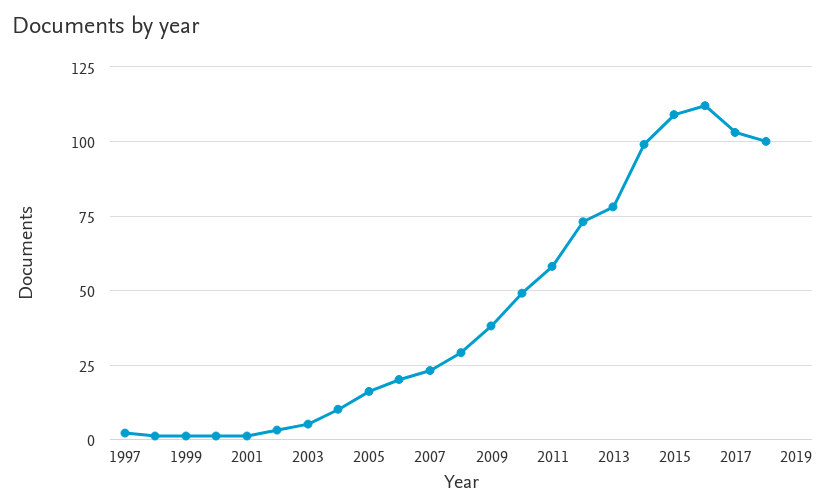
\includegraphics[scale=0.4]{imagenes/scopus-grafico-bioinspirados.png}
	\caption{Gráfico de publicaciones sobre algoritmos bioinspirados registradas en Scopus \cite{scopus-bioinspired}.}
	\label{grafica-scopus}
\end{figure}

Dicha gráfica refleja perfectamente el auge de los algoritmos bioinspirados; de menos de diez publicaciones por año hasta el año 2004 aproximadamente, hasta los más de 100 que llevan registrándose desde 2015. El éxito de estos algoritmos se fundamenta en dos pilares: su carga conceptual es sencilla de abstraer para cualquier usuario, y generalmente aportan buenos resultados a los problemas a los que se han enfrentado.

La principal motivación para construir algoritmos bioinspirados es simple, a la par que consistente: si un ser vivo ha evolucionado durante siglos y siglos hasta llegar a desarrollar una técnica con la que sobrevivir en la naturaleza, dicha técnica debe ser suficientemente óptima como para resultar digna de un estudio. Es por ello que se han propuesto multitud de técnicas que simulan el comportamiento de numerosos seres vivos en su búsqueda de un objetivo.

Actualmente existen algoritmos bioinspirados en cualquier rama del reino animal. Algoritmos de manadas de lobos o grupos de tiburones que acorralan a su presa, basados en bancos de peces que se mueven en grupo hacia una zona óptima, o incluso que simulan el movimiento de una polilla cuando se dirige hacia un foco de luz. Por supuesto, en los años de la explosión de los algoritmos bioinspirados (acorde con la gráfica de la figura \ref{grafica-scopus}, se podría considerar a partir de 2005), con tanta diversidad en las propuestas no tardaron en surgir técnicas cuyo concepto se basaba en un animal muy particular: el ser humano.

\section{Estado del arte: algoritmos socioinspirados}

Conocemos como \textbf{algoritmos socioinspirados} a aquellos que inspiran su funcionamiento en comportamientos basados en la especie humana, y que pueden aplicarse a resolver problemas de cualquier índole. Similar a sus contrapartes bioinspiradas, las técnicas socioinspiradas tienen en el centro de su modelo conceptual a un miembro que forma parte de la naturaleza, en este caso el ser humano, y se aprovechan de sus relaciones, formas de actuar y estilo de vida para intentar dar una solución óptima a un problema.

En el apartado anterior se defendía la investigación de técnicas bioinspiradas por la constante evolución en busca de supervivencia de las distintas especies animales, y esto sucede de forma análoga con las técnicas socioinspiradas. En el caso de estas últimas, sin embargo, la mejora de soluciones no se basa en la evolución genética de la especie a lo largo de los siglos y en la selección natural, sino en el desarrollo de técnicas que permiten a nuestra sociedad alcanzar metas colectivas o individuales. Dichas técnicas pueden resultar cotidianas, pero deteniéndose a analizar cada una de ellas se puede observar que dicho comportamiento se puede trasladar a un algoritmo que explore en un espacio de búsqueda.

Dada la multitud de variedades bioinspiradas que se han propuesto y estudiado desde el surgimiento de dichos algoritmos, era de esperar que se empezasen a valorar técnicas humanas para optimización de funciones. En el día a día de un ser humano suceden cuantiosas situaciones que, sin ser puramente consciente, le obligan a buscar una solución óptima a un problema menor, tales como buscar la ruta más óptima para desplazarse al lugar de trabajo, estimar la máxima cantidad de días que se puede pasar sin realizar la compra o en qué horas debe conectar un electrodoméstico para aprovechar al máximo el consumo energético. Son problemas en los que encontrar soluciones a corto plazo puede resultar trivial, pero las técnicas abordadas en este estudio abarcan temas más complejos, o a mayor escala.

Cabe destacar que son unas técnicas muy recientes, y que a día de hoy ni siquiera existe un estudio formal que analice algunas de las propuestas con experimentos y análisis de rendimiento, como se busca hacer en este Trabajo de Fin de Grado. De hecho, en la actualidad estos algoritmos se encuentran aún en una fase de divulgación y propagación, es decir, los investigadores priorizan buscar nuevas propuestas de algoritmos antes que analizar las ya existentes, bien por falta de ellas o por considerarlas poco prometedoras.

Kumar, Kulkarni y Satapathy \cite{socio-evolution-algorithm} han presentado la última propuesta socioinspirada actual, que data de abril de este mismo año, titulada \textit{Socio evolution \& learning optimization algorithm: A socio-inspired optimization methodology}. En este artículo, antes de explicar su algoritmo, los autores dan una pincelada sobre la situación de los algoritmos socioinspirados. En la gráfica ubicada a continuación se puede observar una clasificación de estos algoritmos, según los autores.

\begin{figure}[h]
	\centering
	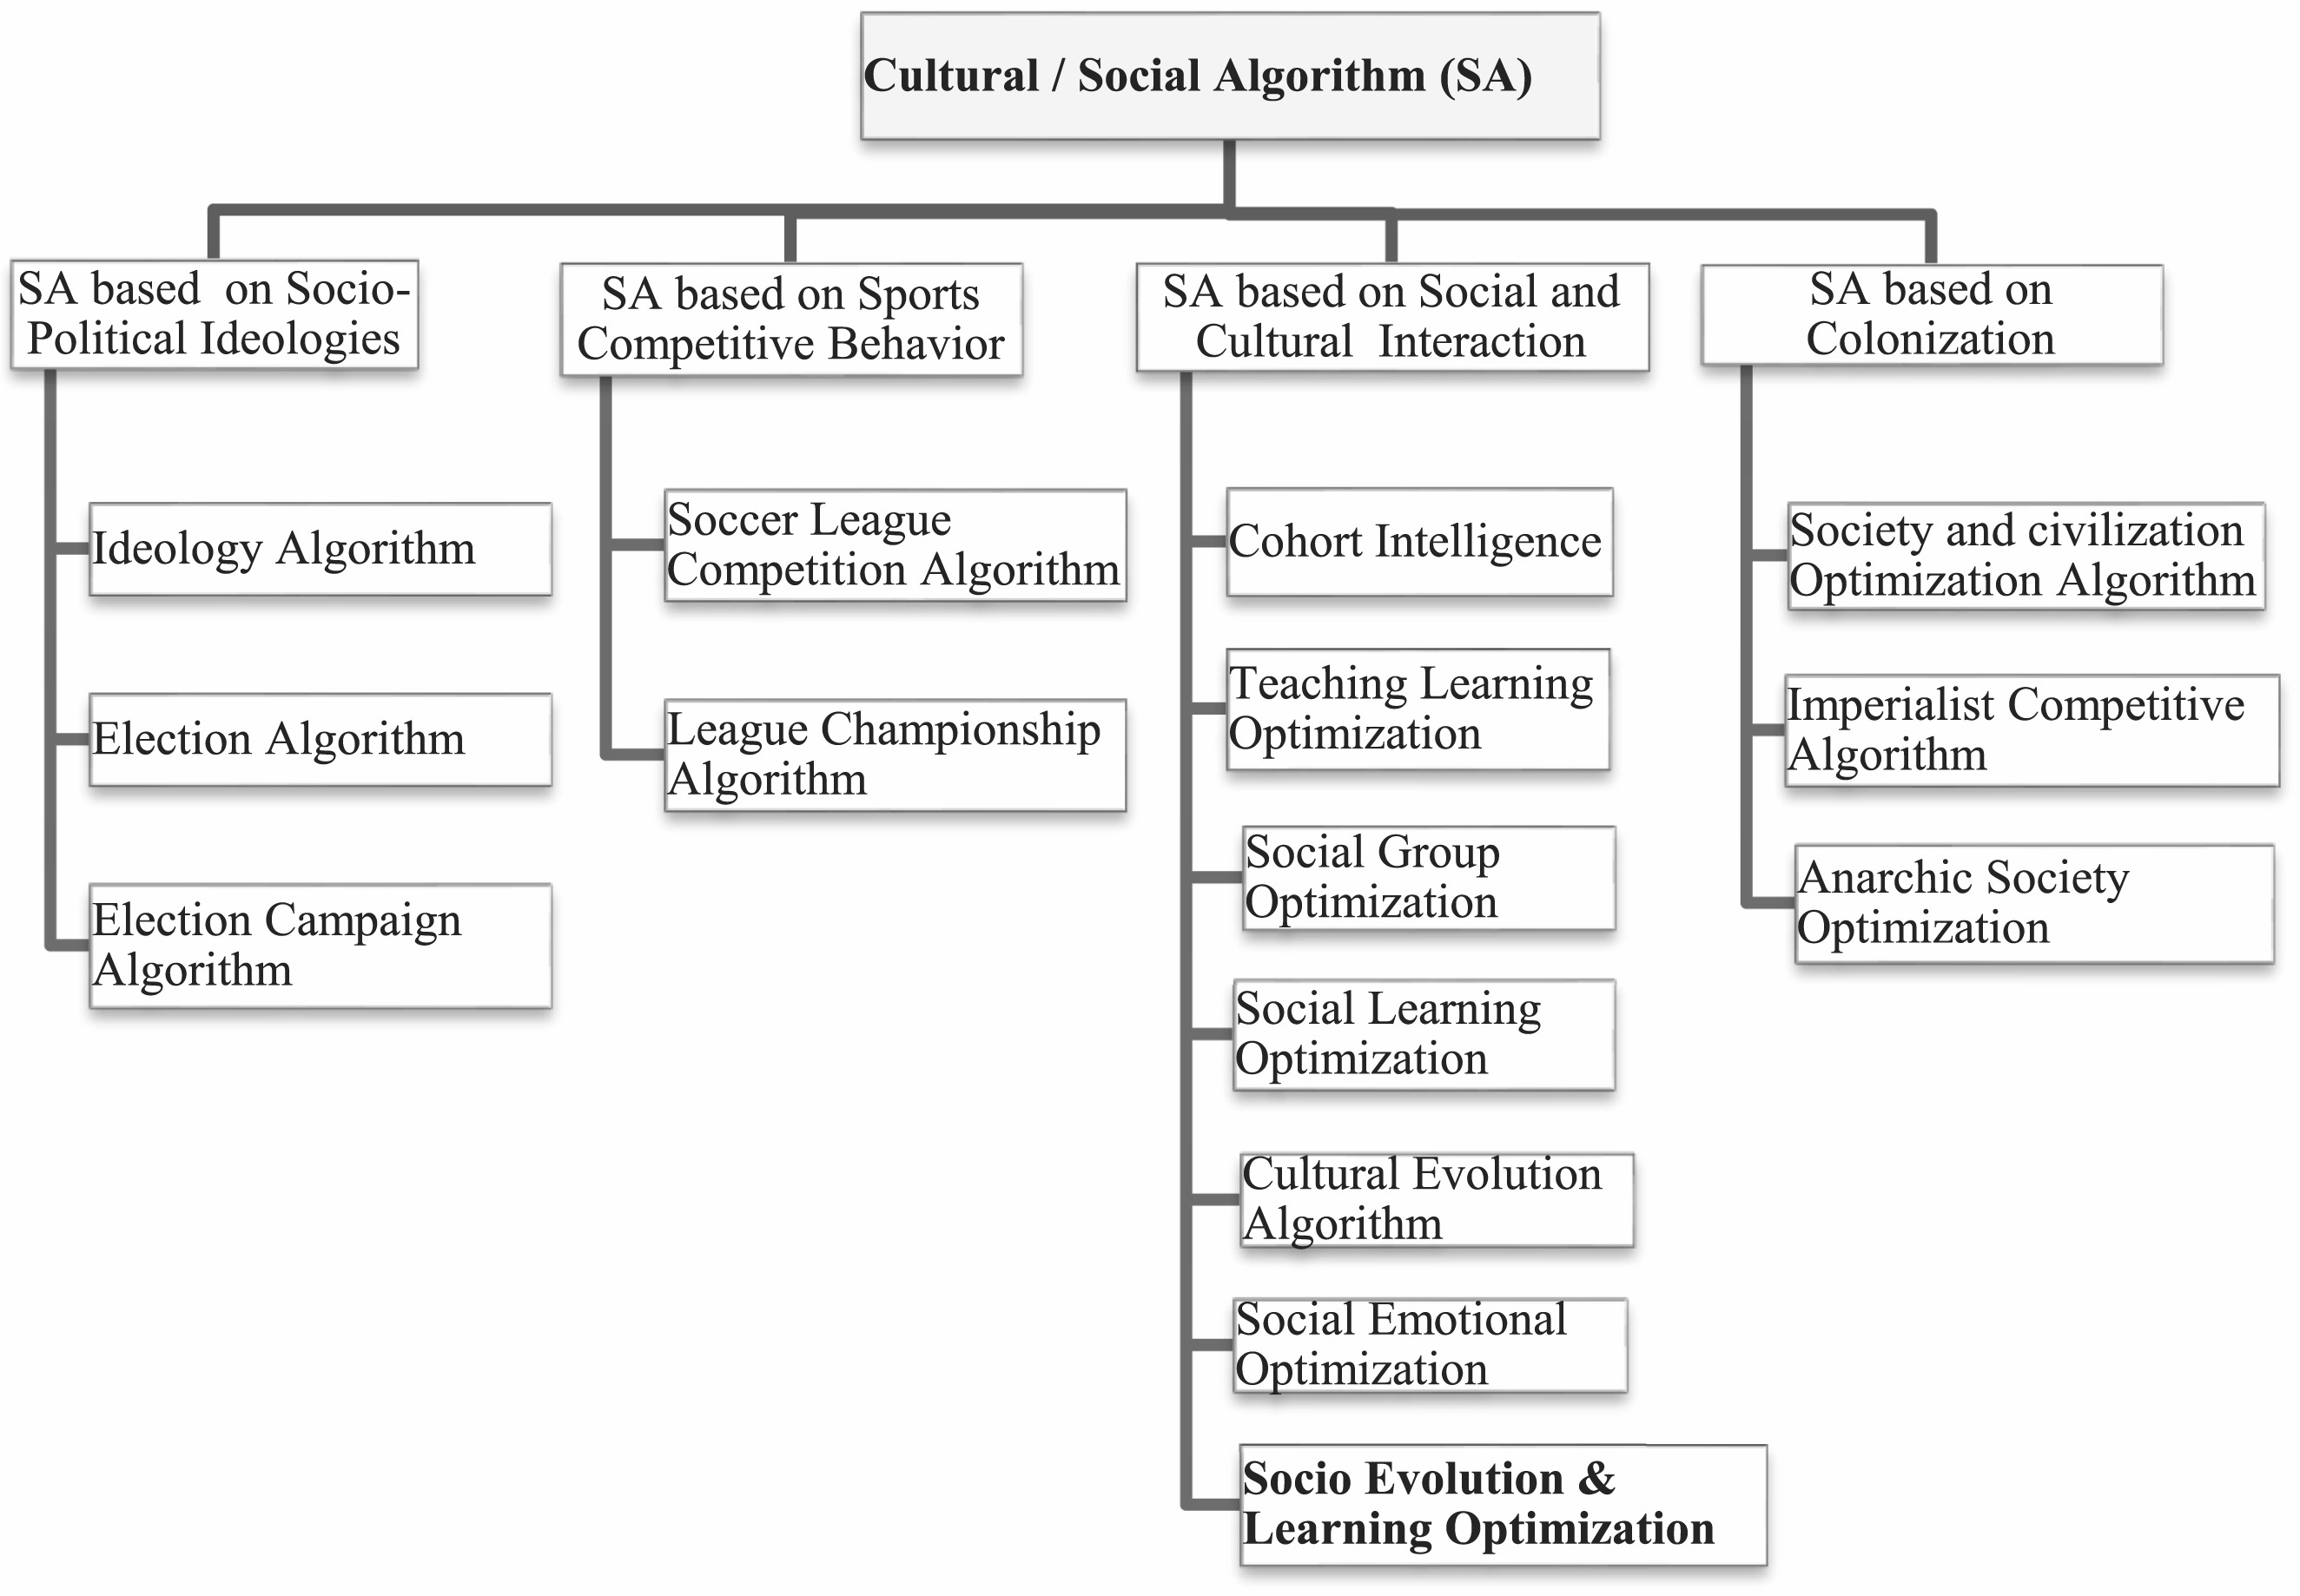
\includegraphics[scale=0.9]{imagenes/socioinspired-classification.jpg}
	\caption{Clasificación estimada de los algoritmos socioinspirados \cite{socio-evolution-algorithm}.}
	\label{clasificacion-socioinspirados}
\end{figure} 

En dicha gráfica se encuentran cinco de los seis algoritmos que son fruto de estudio de este trabajo: del grupo de socioinspirados basados en ideologías socio-políticas, el algoritmo \textit{Ideology Algorithm} (IA) \cite{ia-article}; del grupo de basados en competiciones deportivas, el algoritmo \textit{Soccer League Competition} (SLC) \cite{slc-article}; del grupo de basados en interacción social y cultural, el algoritmo \textit{Social Emotional Optimization Algorithm} (SEA) \cite{sea-chapter}; y del grupo de basados en colonización, los algoritmos \textit{Imperialist Competitive Algorithm} (ICA) \cite{ica-conference} y \textit{Anarchic Society Optimization} (ASO) \cite{aso-article} \cite{aso-chapter}.

El algoritmo restante, que no se muestra en esta gráfica, es \textit{Parliamentary Optimization Algorithm} (POA) \cite{poa-article}, y de haberlo incluido los autores en esta clasificación seguro que estaría en el primer grupo, los basados en ideologías socio-políticas. Su ausencia en la gráfica probablemente se deba al desconocimiento de su existencia por parte de los autores, ya que no es una clasificación muy extensa en la que haya habido necesidad de eliminar información.

Precisamente llama la atención la falta de propuestas en dicha gráfica. Los algoritmos socioinspirados están pasando por la primera etapa de la que se ha hablado en la sección anterior de algoritmos bioinspirados. Las propuestas son innovadoras, llaman la atención, pero pocos investigadores abandonan su campo de trabajo para volcarse con ellas. Poco a poco, si los resultados acompañan, irán desarrollándose nuevas técnicas que, retroalimentándose unas a otras, conseguirán dar consistencia a esta rama de la computación evolutiva.

En palabras de Kumar et al. \cite{socio-evolution-algorithm}, <<estos métodos han ganado popularidad por sus pautas sencillas para buscar soluciones óptimas en problemas computacionales reales y complejos>>. Como se había anticipado en la introducción, esta es la principal motivación para trabajar con algoritmos socioinspirados. Cuando se trata de aproximar a usuarios primerizos a la computación evolutiva, el primer escalón puede ser difícil de sobrepasar. Estos algoritmos aportan una visión más cotidiana, una forma de hacer comprender a casi cualquier persona cómo se puede explorar un espacio de soluciones sin tener que comprender a fondo el contexto de un algoritmo común de estas características.

Hablar de <<población>> en un algoritmo evolutivo no debe suponer ningún problema de comprensión para un investigador dedicado a este campo. Pero resulta mucho más atractivo si a esta población se le da un nombre propio, si se la asocia con un conjunto de individuos que una persona es capaz de reconocer y ubicar. Por ejemplo, con un parlamento político, o con los jugadores de una liga deportiva. Son sólo algunos de los casos que se plantean en los algoritmos estudiados en este trabajo.

Ya que una de las máximas de estos algoritmos es mantener la sencillez y hacer que las técnicas utilizadas sean lo más intuitivas posibles, la metodología que siguen para llegar a una solución óptima también debe ser asociable a conductas reconocibles. Al igual que las poblaciones están compuestas de soluciones habitualmente representadas como <<seres humanos>>, las técnicas evolutivas se corresponden a aquellas acciones realizadas por los mismos para llegar hasta su objetivo. Continuando el símil anterior, realizar debates políticos o jugar partidos de una temporada serían los ejemplos equivalentes.

Dentro de esta metodología siempre hay alguna figura o grupo que sobresale entre la población, y que constituye (o en caso de ser un grupo, contiene) al mejor <<individuo>>. Este se equivaldrá a la mejor solución encontrada para el problema, y es fácilmente reconocible si uno se abstrae a la capa socioinspirada del mismo. El mejor individuo de un parlamento político sería la figura del presidente, o el de una liga deportiva sería el mejor jugador admirado por todo el mundo.

Como se ha podido comprobar, el análisis funcional de los algoritmos socioinspirados es, a diferencia de lo que ocurre con otros algoritmos evolutivos de propósito general, bastante sencillo e intuitivo de transmitir. Esto es claramente debido a la naturalidad con la que un usuario puede asociar dichas pautas a acciones observables en su día a día. No obstante, la eficacia real de estos algoritmos, fuera de las funciones probadas en sus respectivos \textit{papers} o artículos, está aún por probar, ya que de momento no son partícipes de las grandes competiciones acontecidas en congresos, entre las que destacan las del Congress of Evolutionary Computation (CEC).

Sin embargo, sí que se han propuesto en distintas publicaciones algunas aplicaciones de estos algoritmos a resolución de problemas reales muy particulares. En el caso de aquellos algoritmos que se han estudiado en este trabajo, existe una aproximación del algoritmo \textit{Soccer League Competition} para optimizar el diseño de redes de distribución de agua \cite{slc-article}, u otra del algoritmo \textit{Anarchic Society Optimization} para manejar el controlador PID (\textit{proportional–integral–derivative}) de un Regulador de Voltaje Automático (\textit{Automatic Voltage Regulator} o AVR, en inglés) \cite{aso-article}.

Con el paso de los años es de esperar que estos algoritmos sean perfeccionados, sigan evolucionando y se utilicen cada vez en más problemas reales, al igual que sucedió en su momento con los algoritmos bioinspirados.

%
%\chapter{Análisis de los algoritmos}

En este apartado se realizará un análisis detallado sobre cómo funciona cada uno de los algoritmos seleccionados para el estudio desde un punto de vista teórico. Se explicarán las técnicas que utiliza cada uno para llegar a la solución óptima y cómo se asemejan dichas técnicas al comportamiento humano, para de ese modo poder considerarse un algoritmo socioinspirado.

Los algoritmos se analizarán en orden cronológico, siendo el más antiguo de todos Imperialist Competitive Algorithm (2007) \cite{ica-conference} y el más reciente Ideology Algorithm (2016) \cite{ia-article}.

\section{Imperialist Competitive Algorithm (ICA)}

El primer algoritmo a analizar, \textbf{Imperialist Competitive Algorithm} o, según sus siglas, \textbf{ICA}, fue presentado por primera vez en 2007 por Atashpaz-Gargari y Lucas \cite{ica-conference}. Se trata de un algoritmo que podría ser agrupado en la subcategoría de socioinspirados basados en conquistas y colonialismo, como lo han hecho Kumar et al. \cite{socio-evolution-algorithm}.

Este algoritmo parte de la idea de un mundo completamente colonialista, plagado de países que luchan por alzarse vencedores y conquistadores. En esta guerra constante, los países con más poder se volverían los líderes, y podrían contar con numerosas colonias a su servicio. Por otra parte, aquellos países que no pueden vencer a los demás se verían relegados a ocupar un puesto de colonia para siempre.

Durante la guerra también se puede producir una revolución o alzamiento de una de las colonias contra su propio imperio. Si esta colonia resulta ser más poderosa que el actual líder, dicha posición pasa a ser suya. También puede darse el caso totalmente opuesto; si una colonia resulta realmente débil, un imperio colindante puede absorberla y hacerse más fuerte gracias a ella. Y por supuesto, un imperio puede ser colonizado al completo por otro, haciéndose así cargo de sus colonias restantes y del propio país imperial.

En palabras de los propios autores del algoritmo, <<la competición imperialista con suerte convergerá a un estado en el que sólo haya un imperio y todas sus colonias se hallen en la misma posición y tengan el mismo coste que el país imperialista>>.

Como se puede observar de esta hoja de ruta del algoritmo, la relación con la sociedad es evidente, aunque recuerde más a épocas pasadas que a la actualidad. Este es el funcionamiento del algoritmo a grandes rasgos, pero a continuación se detallarán las características más llamativas del mismo. Previamente se muestra un pseudocódigo del algoritmo, para ayudar a comprender cada paso del mismo antes de la explicación detallada.

\begin{algorithm}
	\caption{Imperialist Competitive Algorithm}
	\begin{algorithmic}[1]
		\State $imperios \gets \textit{inicializarImperios()}$
		\While{\textbf{not} \textit{criterioParada}}
		\For{\textbf{each} \textit{colonia}}
		\State $colonia \gets colonia + (imperialista - colonia + rand())$
		\If{$peso(colonia) < peso(imperialista)$}
		\State $imperialista \gets colonia$
		\EndIf
		\EndFor
		\State $imperios \gets competicionImperial()$
		\If{\textbf{any} \textit{imperio} \textbf{is empty}}
		\State $imperios \gets eliminarImperio(imperio)$
		\EndIf
		\EndWhile
		\State{\textbf{return} \textit{min(peso(imperialistas))}}
	\end{algorithmic}
\end{algorithm}

Se puede comenzar este análisis en base a los distintos componentes del algoritmo, relacionándolos con la descripción anterior y comprobando por qué se trata de técnicas socioinspiradas.

En primer lugar conviene hablar acerca de la población. Si bien habitualmente en estos algoritmos socioinspirados la población suele estar constituida de individuos, siendo esta una agrupación de los mismos, en el caso del algoritmo ICA no es así. En este algoritmo se realiza un símil con una sociedad global donde cada una de las soluciones que compone la población es como un país, o en este caso como una colonia. Por tanto, la figura del ser humano como persona individual no aparece en esta propuesta.

Una vez que se han instanciado las primeras soluciones o colonias que ocuparán la población inicial, hay que seleccionar aquellas que sean más poderosas para considerarlas <<imperialistas>>, es decir, serán los líderes de cada uno de los imperios en los que se divida el problema. Por supuesto, tanto el número de colonias como el número de imperios iniciales son definidos en los parámetros del algoritmo y pueden variar si así se desea.

A lo largo de todo este algoritmo se entenderá que un país es más poderoso que otro si \textbf{su evaluación para la función objetivo es menor}, dado que se trata de problemas de optimización buscando el menor valor posible. La asignación de los imperios se hace con respecto a las colonias iniciales con un menor valor para dicha función.

Con los imperios constituidos y las colonias distribuidas se comienza a desarrollar el bucle principal del algoritmo, que finalizará cuando se cumpla el criterio de parada. La implementación de este algoritmo originalmente paraba tras un número de <<décadas>> (iteraciones del bucle principal), pero a fin de integrarlo con el resto de algoritmos del estudio se añadió la posibilidad de definir un criterio de parada por número de evaluaciones de la función objetivo.

En cada iteración de dicho bucle cada colonia realiza un desplazamiento hacia su imperialista. El desplazamiento tiene un componente de aleatoriedad que permite que no converjan todas las soluciones en el primer imperialista nada más comenzar las iteraciones. A continuación se puede observar una representación gráfica de dicho movimiento.

\begin{figure}[h]
	\centering
	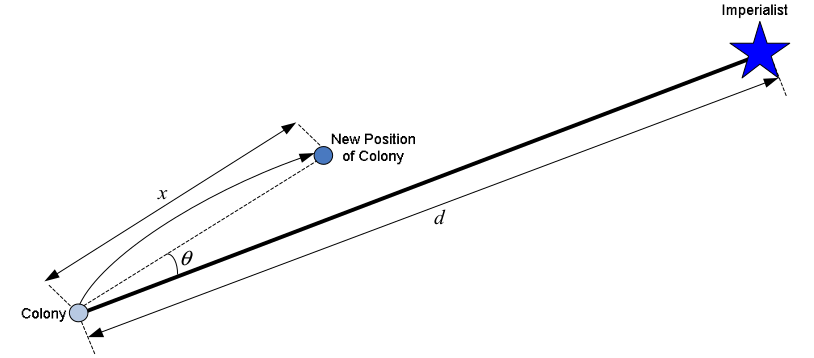
\includegraphics[scale=0.4]{imagenes/ica-desplazamiento.png}
	\caption{Desplazamiento de una colonia hacia su imperialista, con un componente de aleatoriedad \cite{ica-conference}.}
	\label{ica-desplazamiento}
\end{figure}

El movimiento producido $x$ queda definido por la siguiente fórmula

\begin{equation}\label{ica-eq-desplazamiento1}
x \sim U(0, \beta \times d)
\end{equation}

en la cual $d$ es la distancia entre la colonia y el imperialista y $\beta$ representa el llamado <<coeficiente de asimilación>>. Es decir, se trata de un desplazamiento hacia el imperialista donde la distancia recorrida está definida por un valor uniforme aleatorio entre 0 y la máxima distancia.

Además, el ángulo $\theta$ que aparece en la figura, que desvía a la colonia de su dirección, viene calculado de la siguiente forma

\begin{equation}\label{ica-eq-desplazamiento2}
	\theta \sim U(-\gamma, \gamma)
\end{equation}

donde $\gamma$ es el parámetro que ajusta la desviación de la dirección, y que es llamado por los autores <<coeficiente del ángulo de asimilación>>.

Los cambios producidos mediante estos operadores mencionados ayudan a diversificar las posiciones de las colonias y a que no se agrupen automáticamente en torno a la mejor solución del imperio. Esto permite al algoritmo explorar el espacio de búsqueda adecuadamente y no caer en posibles óptimos locales con facilidad en las primeras iteraciones, lo que limitaría mucho el proceso evolutivo. Si la nueva posición hacia la que se mueve una colonia resulta ser mejor que la del actual imperialista de dicho imperio, se intercambian los puestos y el resto de colonias intentará moverse hacia la nueva mejor solución.

La competición imperialista que tiene lugar en cada iteración del bucle principal aporta aún más variedad al proceso, llevando a la peor de las colonias del peor imperio hasta el imperio que más probabilidad tiene de adquirirla, que suele ser el más poderoso. Este poder de los imperios se calcula en función del peso del imperialista y del peso medio de sus colonias. Esta decisión también aporta más variedad a la par que realismo en el proceso imperialista, ya que si un el país líder del imperio es muy poderoso pero tiene muchas colonias débiles, generalmente dicho imperio será menos potente que uno que tenga un imperialista algo peor y menos colonias aunque más fuertes.

Una vez que un imperio se quede sin colonias, este pasa a ser absorbido por el imperio más fuerte, y la cantidad de imperialistas se reduce. El proceso se repite en cada iteración del bucle hasta que quede solamente un imperio que contenga todas las colonias; en tal caso, a partir de esa iteración en el bucle principal solamente se moverán las colonias hacia nuevas posiciones, tratando de explorar las cercanías del país imperialista.

Para concluir el análisis del ICA, se puede afirmar con certeza que basa muchísimo su comportamiento en los algoritmos de \textbf{Particle Swarm Optimization (PSO)}. En este caso, cada imperio funcionaría como un algoritmo PSO en sí, siendo las partículas las colonias y la mejor posición la del país imperialista. La principal variación consiste en que el algoritmo simula varios PSO compitiendo entre sí, aunque mezclando sus partículas mediante revoluciones o intercambiándolas en el proceso. La propuesta es interesante y una de las primeras en aportar un enfoque colonialista al planteamiento del algoritmo, por lo que resultó especialmente interesante para el estudio.

El punto crítico al algoritmo viene en torno a la exploración del espacio de búsqueda. Para ello es necesario distinguir bien en este caso cuál es la fase de exploración y cuál la de explotación. En este algoritmo se produce una exploración del espacio de búsqueda cuando hay varios imperios, y además las colonias del imperio se encuentran suficientemente separadas del imperialista como para que su avance hacia él permita valorar un considerable número de posiciones en los alrededores, pero no en las inmediaciones. Esta búsqueda en las posiciones más cercanas a la mejor solución es la que se considera la explotación, cuyo principal objetivo es comprobar si en las cercanías hay alguna posibilidad de mejora para apuntillar la solución. Esta fase suele darse en las iteraciones más avanzadas del algoritmo, cuando ya se tiene más o menos claro dónde puede estar el óptimo.

Si bien se ha comentado lo interesante de la propuesta para que no se caiga de inmediato en óptimos locales y la ventaja que aporta que cada colonia tenga posibilidad de revolucionarse y dar lugar a una nueva exploración, el problema es que una o dos colonias colocadas de forma aleatoria no suponen una exploración decente. Tener pronto todas las colonias agrupadas en un mismo imperio supone contar con una fase de exploración corta, lo que hace bastante factible la posibilidad de que el algoritmo se quede en un óptimo local y no vuelva a moverse de ahí ya que el resto de las iteraciones implican casi esencialmente una fase de explotación.

\section{Parliamentary Optimization Algorithm (POA)}

El segundo algoritmo en la lista cronológica es \textbf{Parliamentary Optimization Algorithm}, o \textbf{POA} acorde a sus siglas, que fue presentado en 2008 \cite{poa-article} en la revista \textit{International Journal of Innovative Computing, Information \& Control}, también conocida como \textit{IJICIC}. Este algoritmo está englobado en el apartado de socioinspirados basados en ideologías socio-políticas, obviamente en la vertiente de políticas.

Esta propuesta simula ubicarse dentro de un marco político, en un parlamento. En el mismo tendrán cabida una serie de partidos políticos que tratarán de hacerse con el control del gobierno. Dentro de cada uno tendrá lugar una competición por ascender hasta los puestos de candidato del partido, donde los distintos miembros pueden evolucionar hasta parecerse a sus candidatos, y si alguno de ellos aporta soluciones diferentes y mejores, incluso sucederles en el cargo.

Constantemente se producen también una serie de debates políticos que pueden llevar a los partidos más minoritarios a desaparecer del parlamento, o a algunos de los más votados a confluir y unirse en un pacto para asegurarse estar presentes en el gobierno. Entre todos los candidatos aportados por cada partido se escoge como presidente del parlamento a aquel que sea considerado el mejor político. En caso de que haya un único partido o confluencia, se escoge igualmente al mejor representante de dicha agrupación.

Este algoritmo tiene un funcionamiento sencillo pero a la vez es muy intuitivo de asociar con la sociedad, ya que se ubica en un entorno muy habitual y cotidiano. La política está presente en prácticamente cada acto de la vida diaria y la estructura de un parlamento es por todos conocida. En todo caso, los debates políticos que allí acontecen son accesibles para cualquier ciudadano y es común entender cómo funcionan y cómo se desenvuelven los partidos políticos para ganar escaños y hacerse con las elecciones.

A continuación se incluye un pseudocódigo del algoritmo para comprender de forma general cuál es el funcionamiento en cuanto a pasos a seguir y procedimientos.

\begin{algorithm}
	\caption{Parliamentary Optimization Algorithm}
	\begin{algorithmic}[1]
		\State $parlamento \gets \textit{inicializarPartidos()}$
		\State $candidatos_{partido_i} \gets mejoresMiembros(partido_i)$
		\While{\textbf{not} \textit{criterioParada}}
		\For{\textbf{each} \textit{partido}}
		\State $miembro_i \gets (candidatos_{partido} - miembro_i) \times bias$
		\If{$peso(miembro_i) < peso(candidato_{j,partido})$}
		\State $candidato_{j,partido} \gets miembro_i$
		\EndIf
		\State $poder_{partido} \gets computarPoder(partido)$
		\EndFor
		\State{\textbf{confluir los 2 mejores partidos con probabilidad} $p_m$}
		\State{\textbf{eliminar el peor partido con probabilidad} $p_d$}
		\EndWhile
		\State{\textbf{return} \textit{min(peso(candidatos))}}
	\end{algorithmic}
\end{algorithm}

Se empezará a analizar este algoritmo relacionando los conceptos técnicos presentados en este pseudocódigo con la descripción en lenguaje natural realizada previamente.

En el caso de esta propuesta, la población inicial está compuesta de soluciones que se interpretan como individuos humanos. A lo largo de este algoritmo se asociará cada una de las soluciones con un político particular, y su evaluación en la función objetivo del problema determinará lo válido que es dicho político dentro del parlamento.

Con los primeros políticos generados, este algoritmo los agrupa por partidos, tantos como se haya indicado en los parámetros del mismo. Además, el algoritmo recibe como parámetro el número de candidatos que tiene cada partido, así que debe seleccionar de entre los mejores políticos tantos como candidatos haya, para asignarlos a los distintos grupos parlamentarios. Estos se repartirán equitativamente el resto de miembros del parlamento, para partir desde una situación de igualdad.

En este punto ya se ha generado la situación inicial del problema, y se procede a entrar en el bucle principal. En cada iteración primero se produce una competición interna dentro del propio partido, y después se da pie a una cooperación entre partidos que puede llegar a buen puerto o no.

La competición interna consiste en mover todos los políticos hacia sus candidatos, con un sesgo determinado que evite una congregación de todo el partido en un único punto. Para ello se sigue la siguiente fórmula

\begin{equation}\label{poa-eq-desplazamiento}
	p' = p_0 + \eta(\frac{\sum_{i=1}^{\theta}(p_i - p_0) \times f(p_i)}{\sum_{i=1}^{\theta}f(p_i)})
\end{equation}

donde:

\begin{itemize}
	\item $p'$ es la nueva posición
	\item $p_0$ es la posición actual del político
	\item $p_i$ representa a cada candidato del partido
	\item $\eta$ es el sesgo que se aplica al movimiento
	\item $f(p)$ es la evaluación de la función objetivo para el político $p$
	\item $\theta$ es el número de candidatos por partido
\end{itemize}

Lo importante en este algoritmo es que, según viene especificado en la propia descripción del mismo, el desplazamiento únicamente tiene lugar \textbf{si la nueva posición es mejor que la anterior.} Si en el proceso de desplazamiento algún político resulta estar mejor ubicado que alguno de los actuales candidatos, estos intercambian sus puestos y el anterior miembro regular del partido pasa a ser un nuevo candidato. De esta forma el resto de los políticos en futuras iteraciones se desplazarán hacia esta nueva solución.

Cuando termina la competición interna del partido, se produce la fase de cooperación. En este momento existen dos parámetros $p_m$ y $p_d$ que simbolizan la probabilidad de que los dos mejores partidos se unan (\textit{merge}) y de que el peor partido sea expulsado del parlamento (\textit{delete}), respectivamente. En caso de que se dé la primera condición probabilística, los dos mejores partidos dejan a un lado sus diferencias y confluyen en uno solo, escogiendo como candidatos a los mejores miembros entre ambos partidos sin importar su partido de origen. Si por otro lado, se produce el segundo caso, el partido es eliminado del parlamento y todos los miembros desaparecen del mismo, por lo que el parlamento ve reducido su tamaño, haciendo hincapié en las mejores soluciones para el resto de sus iteraciones.

Este algoritmo basa su funcionamiento en el \textbf{Particle Swarm Optimization} o \textbf{PSO}, comportándose de manera muy similar pero dando un carácter socio-político al entorno del mismo. En este caso cada partido funciona como un algoritmo PSO, siendo los políticos las partículas y los candidatos aquellas situadas en mejor posición a las que el resto se acercan. En cada iteración la posibilidad de hacer confluir dos partidos puede permitir aumentar la exploración, entendiéndose que un político puede optar a acercarse a un candidato que antes no conocía, y por el camino explorar una zona desconocida.

La principal novedad que aporta este algoritmo con respecto al PSO es la de tomar como referencia de desplazamiento un número mayor de partículas, en particular el que se desee y se especifique en la llamada al algoritmo. Esto permite que se puedan generar más de una <<buena posición>> hacia la que dirigirse, explorando también los caminos intermedios.

La crítica a este algoritmo se basa en la forma de realizar el desplazamiento, que limita la exploración. Al no permitir que las partículas pasen a ocupar una peor posición se puede caer fácilmente en un óptimo local si se estabilizan en las primeras iteraciones. Además, el sesgo es un parámetro fijado según han documentado los propios autores \cite{poa-article} y eso resta aleatoriedad a la búsqueda y puede frenarla totalmente en un determinado punto en el que siempre se realice el mismo desplazamiento y ninguna partícula mejore su posición.

\section{Social Emotional Optimization Algorithm (SEA)}

El siguiente algoritmo de esta lista en orden cronológico es el \textbf{Social Emotional Optimization Algorithm}, o \textbf{SEA} de acuerdo a las siglas elegidas por los autores \cite{sea-chapter} para representarlo. Esta propuesta se presentó en 2010 en el libro \textit{Swarm, evolutionary, and memetic computing. First international conference on swarm, evolutionary, and memetic computing, SEMCCO} \cite{sea-book}. Este algoritmo podría ser englobado en la subcategoría de socioinspirados basados en interacción social y cultural según Kumar et al. \cite{socio-evolution-algorithm}.

Esta técnica socioinspirada está fundada en las relaciones sociales de las personas y cómo reaccionan en función de sus aciertos y errores o de la forma de actuar de los demás. Para ello hay que tener en cuenta las acciones pasadas y cómo influyeron en el resto de la sociedad, y a su vez comprobar cómo influye en un individuo el comportamiento de los demás.

En cuanto a esto, es de esperar que si un individuo ve que el resto de la sociedad encuentra posiciones mejores a la suya, su índice de emoción disminuya, al igual que aumenta por completo si se coloca como el individuo con mejor posición en toda la población. Al principio todos los individuos comienzan con la moral al mismo nivel, pero esta variará dinámicamente en función de los resultados que se vayan obteniendo.

Cuando llega el momento de que cada individuo realice su siguiente movimiento, tiene tres posibles formas de hacerlo:

\begin{itemize}
	\item Si su moral está muy alta porque es consciente de que tiene una buena posición, su movimiento simplemente le lleva a alejarse de las peores posiciones a la par que se fija en su mejor posición histórica.
	\item Si su moral es media porque aún está algo conforme consigo mismo a pesar de que sabe que puede mejorar, se alejará de las peores posiciones a la vez que busca un movimiento hacia la mejor posición que él mismo ha tenido y la mejor posición registrada por la población hasta ese momento.
	\item Si su moral es muy baja porque es conocedor de lo mala que es su posición, buscará inspirarse en la mejor solución de la población hasta el momento.
\end{itemize}

El paso del tiempo da lugar a que las distintas soluciones evolucionen y sepan el lugar al que pertenecen dentro de la sociedad. En el siguiente pseudocódigo se puede ver con más claridad cómo funciona el algoritmo.

\begin{algorithm}
	\caption{Social Emotional Optimization Algorithm}
	\begin{algorithmic}[1]
		\State $sociedad \gets \textit{inicializarPoblacion()}$
		\State $emocion_i \gets 1.0$
		\State $sociedad_i \gets comportamiento\textit{1}()$
		\While{\textbf{not} \textit{criterioParada}}
		\If{$emocion_i > \textit{limite1}$}
		\State $sociedad_i \gets comportamiento\textit{4}()$
		\ElsIf{$limite2 > emocion_i \ge \textit{limite1}$}
		\State $sociedad_i \gets comportamiento\textit{3}()$
		\Else
		\State $sociedad_i \gets comportamiento\textit{2}()$
		\EndIf
		\If{$peso(sociedad_i) < peso(minimoHistorico) $}
		\State $emocion_i \gets 1.0$
		\Else
		\State $emocion_i \gets emocion_i - \Delta$
		\EndIf
		\State{\textbf{actualizar mejores posiciones históricas}}
		\EndWhile
		\State{\textbf{return} \textit{peso(minimoHistorico)}}
	\end{algorithmic}
\end{algorithm}

Se puede empezar el análisis del algoritmo entendiendo cómo se representan técnicamente la población y los distintos componentes observados en el pseudocódigo, y por tanto cómo se pueden relacionar los mismos con una técnica socioinspirada.

En primer lugar, la población representa una sociedad de seres humanos, donde cada uno de los individuos de la misma es una solución al problema, generada aleatoriamente para la población inicial. En esta sociedad será donde los individuos crezcan intentando ser mejores y situarse por encima del resto. El índice de emoción de cada individuo será un valor real entre 0 y 1, siendo 1 para todos los individuos al inicio del algoritmo. El índice aumentará o decrecerá en función de los éxitos o los fracasos del individuo con respecto a sí mismo y al resto de la población.

En la primera iteración del algoritmo, como todos los índices están a 1, se produce un movimiento especial que no tiene lugar en el resto del proceso. Este movimiento simplemente aleja al individuo de las peores posiciones que hay actualmente en la población, como mecanismo de defensa para no acabar en una situación como esa. Las soluciones a las que les haya tocado caer en las peores posiciones verán sus índices de emoción reducidos hasta que logren desplazarse a una zona mejor siguiendo el camino de un individuo con éxito.

Este algoritmo guarda una posición histórica para cada individuo, la mejor que ha conseguido a lo largo de las iteraciones. Esta posición se usará tanto para las fórmulas de desplazamiento como para guardar la mejor solución hasta el momento, ya que este algoritmo no es elitista y permite que las mejores soluciones se pierdan de la población actual. Guardándolas se asegura sin embargo poder obtener la mejor solución encontrada a lo largo de las iteraciones cuando haya que devolver el valor final del proceso.

Cada vez que se realiza un movimiento, el índice de emoción del individuo cambia. Si el movimiento le coloca en la mejor posición histórica, su emoción aumenta hasta el máximo valor, mientras que si no lo consigue dicho índice se verá decrementado en un parámetro $\Delta$ definido previamente con el algoritmo. En función de la emoción del individuo, en cada iteración optará por seguir un comportamiento u otro a la hora de desplazarse. Un comportamiento u otro queda determinado por unos límites que dividen el dominio del índice, [0,1], en tres secciones. Para ello son necesarios dos límites, que se definen como parámetros del algoritmo.

El SEA puede ser interpretado como un \textbf{Particle Swarm Optimization (PSO)}, al que se le han realizado algunas modificaciones, como la memoria de posiciones históricas y la variación del comportamiento en función del índice de emoción. La idea de tener un comportamiento distinto adecuado a la situación en el tiempo de cada solución es muy interesante y da lugar a múltiples ideas que pueden mejorar esta técnica. Como algoritmo socioinspirado, este intenta darle un significado con sentido a la toma de decisiones de los individuos, para que cada rango de valores del índice de emoción corresponda a un comportamiento u otro.

Al final, sin embargo, el proceso sigue siendo el mismo que en un PSO en el que las partículas (individuos) buscan acercarse a la que saben que es la mejor, aunque en este caso esta puede ser la mejor histórica y no estar presente en la población del momento. La crítica a este algoritmo recae en el manejo de los índices de emoción, ya que es muy fácil que decaigan si se ha llegado a un óptimo local ya que el algoritmo en ningún momento volverá a explorar lejos de ese punto. Si todas las soluciones posteriores resultan son peores que aquella que ha ocupado el puesto de mejor histórica los índices de todos los individuos decaerán hasta el 0, y por tanto se limitarán a buscar en los alrededores de dicho óptimo local.

\section{Anarchic Society Optimization (ASO)}

El algoritmo \textbf{Anarchic Society Optimization}, por sus siglas \textbf{ASO}, fue presentado por primera vez en 2011 por Ahmadi Javid \cite{aso-conference} en el Congress of Evolutionary Computation (CEC). A partir de ese momento se ha utilizado este algoritmo para resolver algunos problemas reales, como este \cite{aso-article}.

Esta técnica ha sido agrupada por Kumar et al. \cite{socio-evolution-algorithm} en el subapartado de socioinspiradas basadas en colonización. Sin embargo, de acuerdo al análisis que se ha realizado para este estudio se ha determinado que un mejor grupo para él sería el de ideologías socio-políticas, y en la siguiente explicación se exponen los argumentos.

ASO es un algoritmo basado en una sociedad anarquista, en la que la figura del gobierno no es necesaria y donde los propios individuos se organizan a sí mismos. Por separado o mediante grupos, podrán determinar cuál es el la mejor decisión posible en cada caso en base a sus propias experiencias y a las del resto de la sociedad.

Para ello, cada individuo tiene que tomar una decisión cuando realice un movimiento: tiene que valorar si le conviene más basarse en su propia situación, en las experiencias del resto de la sociedad actual o en lo que ocurrió en el pasado. Si realiza esta comparación de forma equilibrada y aprovechando toda la información de la que dispone (se supone que en esta sociedad el individuo está al tanto de las decisiones que toman el resto) podrá llegar hasta una posición más favorable, o incluso óptima.

Además, los individuos de una sociedad anárquica pueden experimentar cambios radicales de parecer y dirigirse hacia posiciones que no tienen por qué ser necesariamente mejores. En palabras del propio autor original, los individuos <<también se comportan aventurada e irracionalmente, moviéndose hacia posiciones inferiores que ya han visitado>>. 

Cuando han valorado todas las posibilidades de movimiento según las directrices indicadas anteriormente, los individuos deciden qué estrategia seguir para tomar su nueva posición. Pueden quedarse con la estrictamente mejor de las soluciones planteadas o bien intentar escoger lo mejor de cada una de ellas.

A lo largo del tiempo se espera que al menos un buen porcentaje de la sociedad haya aprendido las buenas conductas y descubra la zona del espacio donde mejor ubicados pueden estar, aunque haya otros miembros que no lo tengan tan claro y deambulen por el resto del espacio explorando diferentes rutas. Al final resulta ambicioso esperar que toda la sociedad converja en un mismo punto, y es normal que se produzcan escisiones así, como bien representa el algoritmo.

A continuación se muestra un pseudocódigo que ayuda a expresar este proceso en términos más cercanos a la implementación.

\begin{algorithm}
	\caption{Anarchic Society Optimization}
	\begin{algorithmic}[1]
		\State $sociedad \gets \textit{inicializarPoblacion()}$
		\While{\textbf{not} \textit{criterioParada}}
		\State $Mp^{current}_i \gets movimientoBasadoEnPropiaPosicion()$
		\State $Mp^{society}_i \gets movimientoBasadoEnSociedad()$
		\State $Mp^{past}_i \gets movimientoBasadoEnHistoria()$
		\State $sociedad_i \gets seleccionMovimiento(Mp^{current}_i, Mp^{society}_i, Mp^{past}_i)$
		\State{\textbf{actualizar mejores posiciones históricas}}
		\EndWhile
		\State{\textbf{return} \textit{peso(minimoHistorico)}}
	\end{algorithmic}
\end{algorithm}

Este algoritmo no es muy complejo en cuanto a instrucciones se refiere, sin embargo a continuación se analizará cómo se ha implementado la propuesta y qué decisiones se han tomado.

En primer lugar es conveniente notar que todo el peso de este algoritmo recae sobre las decisiones de movimiento dado que es realmente lo que tiene carga de trabajo en cada iteración. Este algoritmo solamente debe mantener la mejor posición que cada individuo ha conseguido hasta esa iteración y utilizar tres fórmulas matemáticas que determinen la nueva posición acorde a cada movimiento. La cuestión es averiguar si dichas fórmulas son suficiente para hallar una solución óptima en el espacio de búsqueda.

El movimiento basado en su situación actual viene determinado por un parámetro definido como el autor como <<inestabilidad>> (\textit{fickleness}) o tendencia al cambio. Un valor bajo de este atributo indicará al individuo que debería seguir explorando el espacio por sus cercanías, mientras que un valor alto repercutirá en que actúe de forma individualista y cambie radicalmente de posición.

En el movimiento basado en el resto de la sociedad influye, por supuesto, la mejor solución que el individuo puede encontrar en la iteración actual. Él conoce la posición del resto de sus compañeros, y sabe en quién debe fijarse, pero en lugar de automáticamente copiarlo calcula un <<índice de irregularidad externa>>. De nuevo existe un umbral relacionado con este índice que determina si el individuo debe proceder a desplazarse hacia la mejor posición de la iteración actual o por el contrario se rebela y actúa por su cuenta generando una posición alejada de la misma.

Por último, el movimiento basado en el registro histórico es muy similar al que se acaba de explicar. En este caso la posición en la que el individuo se fija no es la mejor actual sino la mejor histórica, y el índice calculado se denomina <<índice de irregularidad interna>>. Existe también un umbral análogo, solamente que en este caso el desplazamiento se realiza lógicamente hacia la mejor posición que ha habido en todas las iteraciones.

Con todos los posibles movimientos evaluados, el individuo debe tomar una decisión. En este punto entra el operador de selección para elegir con qué movimiento se queda, y la definición del algoritmo en el \textit{paper} original aporta dos posibles soluciones: que se elija según un modelo \textbf{elitista}, quedándose con la mejor posición de las tres generadas, o que se elija según un modelo \textbf{secuencial}, y en cada iteración cambie de uno a otro siguiendo la misma serie. Cada uno tiene sus ventajas e inconvenientes, que además son principalmente excluyentes del otro método. En el caso elitista se consumen muchas evaluaciones de la función objetivo, el triple que en otro algoritmo evolutivo común, pero sin embargo se produce una exploración del espacio más variada. En el caso secuencial tan sólo se producen una tercera parte de las evaluaciones, pero estas no dan la seguridad de ser la mejor en cada caso. En lo que a la implementación de este estudio corresponde, se ha optado por desarrollar la opción \textbf{elitista}.

Este algoritmo también basa su funcionamiento en un \textbf{Particle Swarm Optimization (PSO)}, ya que hasta el propio autor dedica un apartado a la comparación del ASO con el PSO \cite{aso-conference}. En dicho apartado hace una similitud entre los vectores de velocidad del PSO y los movimientos basados en cada uno de los comportamientos anteriormente descritos. En general, asemeja la forma de desplazarse de cada uno de los algoritmos buscando en cada caso del ASO un objetivo distinto dependiendo del movimiento escogido.

\section{Soccer League Competition (SLC)}

El siguiente algoritmo en orden cronológico es el \textbf{Soccer League Competition}, \textbf{SLC} según sus siglas. Fue presentado en 2014 por Moosavian y Kasaee Roodsari \cite{slc-nonlinear-eq}, en una propuesta para resolver ecuaciones no lineales. Más adelante el propio Moosavian ha presentado otras publicaciones aplicando este algoritmo a problemas de la mochila (\textit{knapsack problems}) \cite{slc-knapsack} y a un problema más real, como la distribución de agua en una red \cite{slc-article}. El algoritmo puede ubicarse en el subapartado de socioinspirados basados en comportamiento competitivo, según Kumar et al. \cite{socio-evolution-algorithm}

En este algoritmo se ubica el problema en un marco deportivo, en particular en una liga de fútbol. La población está constituida por equipos, cada uno de ellos con sus diferentes jugadores. A su vez, se distingue entre jugadores titulares y suplentes, y unos lógicamente tienen más importancia que los otros. En este panorama el objetivo de cada jugador es llegar a ser el mejor de la liga, o en su defecto al menos ser lo suficientemente bueno como para que los mejores equipos de la competición quieran contar con él en su plantilla.

Los equipos compiten entre sí a lo largo de temporadas, y los jugadores mejoran en función de su resultado en los partidos, y de la influencia que hayan tenido en el juego. Un jugador titular mejorará más que uno suplente, y si algún titular baja el nivel puede ser relegado al banquillo. A su vez, si un jugador suplente no da la talla para el equipo, este puede despedirle y fichar un nuevo recambio para el próximo partido. El movimiento dicta que los titulares buscan parecerse al \textit{<<Super Star Player>>} para optar a jugar en mejores equipos, mientras que los suplentes intentan llegar al nivel medio de los titulares de su equipo, a fin de encontrar un puesto en la rotación. Con respecto al equipo perdedor, un porcentaje de sus jugadores intentará entrenar alguna nueva técnica con la que vencer a ese equipo en el próximo partido.

Cuando acaba la temporada los mejores equipos se hacen con los mejores jugadores, dejando los peores para los equipos más humildes. Así, la siguiente temporada los jugadores más prometedores pueden seguir mejorando al estar rodeados de un entorno a su altura, y los humildes pueden destacar dentro de su propio equipo, pudiendo llegar a llamar la atención de uno más potente. El mejor jugador, o \textit{<<Super Star Player>>} según el autor, será el que el algoritmo devuelva como resultado de todas las temporadas.

A continuación se muestra un pseudocódigo del algoritmo que explique de manera más técnica los detalles que lo rodean.

\begin{algorithm}
	\caption{Soccer League Competition}
	\begin{algorithmic}[1]
		\State $liga \gets \textit{inicializarLiga()}$
		\While{\textbf{not} \textit{criterioParada}}
		\For{\textbf{each} \textit{par($equipo_i, equipo_j$)}}
		\State $vencedor, perdedor \gets partido(equipo_i, equipo_j)$
		\State $titulares_{vencedor} \gets operadorImitacion()$
		\State $suplentes_{vencedor} \gets operadorProvocacion()$
		\EndFor
		\State{\textbf{reordenar jugadores en función de su fitness}}
		\If {$condicionDescenso$}
		\State $equipo_{peor} \gets nuevoEquipo()$
		\EndIf
		\EndWhile
		\State{\textbf{return} \textit{peso(superStarPlayer)}}
	\end{algorithmic}
\end{algorithm}

Con este pseudocódigo comprendido, se procede a relacionar el comportamiento explicado anteriormente con las instrucciones que se muestran, así como a asociar cada uno de los componentes a su contraparte socioinspirada.

En primer lugar la población en este caso está compuesta de jugadores. Ellos son los que representan las soluciones al problema, y que irán evolucionando conforme el proceso algorítmico tenga lugar. Esta población se divide en equipos, cada uno de los cuales cuenta con sus propios jugadores, y dicha plantilla con jugadores titulares y jugadores suplentes. Los titulares serán las mejores soluciones del equipo y los suplentes aquellas no tan buenas.

Las soluciones deben estar ordenadas en cada <<temporada>> (que corresponde a una iteración del bucle principal), por lo que el primer equipo de la liga siempre empezará la temporada con los mejores jugadores, mientras el último será el que se quede con los peores. Sin embargo, a mitad de cada temporada puede darse el caso de que un jugador de un equipo más humilde llegue a dar una solución suficientemente buena como para ocupar las mejores posiciones de la liga. En dicho caso, este jugador será fichado por el mejor equipo cuando termine la temporada.

El proceso de la temporada consiste en que cada equipo juegue un partido contra el resto de equipos, y en función del resultado sus jugadores mejorarán de una u otra manera. Este partido se simula calculando el coste de cada equipo participante, estimando la probabilidad de cada uno para salir vencedor, y a continuación se genera un valor aleatorio que determine qué equipo es el que gana.

Los jugadores titulares del equipo ganador realizan un movimiento hacia el mejor jugador de la liga, el \textit{<<Super Star Player>>}. Si dicho movimiento no supone una mejora, realizan un movimiento hacia el \textit{<<Star Player>>} de su propio equipo, es decir, su mejor jugador. En caso de que tampoco se encuentre una mejora, intenta hacer un último movimiento aleatorio hacia una posición totalmente distinta. Si el resultado sigue sin mejorar, el jugador no se mueve a consecuencia de ese partido.

Los jugadores suplentes del equipo vencedor deben intentar parecerse a los jugadores titulares, con esperanza de ocupar su puesto. Para ello se introduce el operador de gravedad, que aplicado a los jugadores titulares del equipo representa la posición media que ocupan en el espacio de búsqueda. Ese será el punto al que el jugador suplente intente desplazarse. En caso de que no dé un buen resultado, realiza un movimiento similar a la inversa, alejándose de ese centro de gravedad. Si este movimiento tampoco supone una mejora a la posición inicial el jugador es despedido del equipo y un nuevo suplente generado aleatoriamente ocupa su lugar.

Con respecto al equipo perdedor, el \textit{paper} original no especifica nada, y sin embargo el código MATLAB descargado \cite{slc-matlab} incluye una ligera mutación que aporta variedad al proceso de búsqueda. Esta modificación ha sido plasmada en la implementación de este estudio, y se basa en seleccionar tres miembros de la plantilla titular y mutar un porcentaje de sus componentes. Solamente si la mejora resulta mejor que el original, la mutación queda registrada. A continuación se seleccionan dos suplentes de dicho equipo perdedor y se genera un cruce genético entre ellos, obteniendo dos nuevas soluciones. El equipo reordena su plantilla y se queda con los mejores jugadores de todos los generados, liberando a los peores.

Finalmente, al final de la temporada los jugadores vuelven a ser ordenados, pero esta vez a nivel global, lo que simula el fichaje de los mejores jugadores por el mejor equipo. Los suplentes del primer equipo son mejores que los titulares del segundo equipo, y así sucesivamente, planteando una liga donde claramente existe un equipo con suficiente poder adquisitivo para hacerse con todos los mejores jugadores. Si se ha especificado el componente de descenso, cuando se haya cumplido la condición necesaria el peor equipo queda eliminado de la competición y es rellenado con nuevos jugadores generados aleatoriamente, a fin de aportar mayor exploración a lo largo de todo el proceso.

(Incluir aquí conclusión final de SLC relacionándolo con un algoritmo evolutivo, ¿PSO?)

\section{Ideology Algorithm (IA)}

Por último, el algoritmo socioinspirado más reciente del estudio es el \textbf{Ideology Algorithm}, también referido como \textbf{IA} por sus siglas. Se trata de un algoritmo presentado por Ting Huan et al. \cite{ia-article} en 2016, por lo que se puede considerar muy actual en el momento de redacción de este trabajo. En su agrupación de algoritmos socioinspirados, Kumar et al. \cite{socio-evolution-algorithm} lo clasifican en el grupo de los basados en ideologías socio-políticas.

Esta propuesta parte de una idea similar a la del algoritmo \textbf{POA} \cite{poa-article}, presentado previamente en este mismo capítulo, ya que también tiene lugar en un contexto político en el que distintos partidos tratan de hacerse con el control del gobierno. Estos están representados por un líder, el que se equiparía al presidente del partido, aunque la figura del vicepresidente, o segundo mejor miembro del partido, también juega un papel fundamental.

En este algoritmo, el líder tiene que intentar mantenerse al frente de su partido a la par que intenta ascender hasta colocarse como presidente del gobierno. Para esto pasa por tres fases, una de introspección, otra de competición local y una tercera de competición global. Durante la fase de introspección, el líder del partido busca en torno a su actual posición para intentar mejorar de cara a la siguiente fase. Durante la competición local busca en torno al segundo mejor político de su partido, al vicepresidente, para intentar mantener su puesto y adelantarse a un posible movimiento futuro de este. Por último, en la competición global el líder calcula un movimiento similar a los anteriores pero con respecto al actual presidente del gobierno. Una vez que ha valorado todos los movimientos, selecciona uno utilizando el método de la ruleta (\textit{<<Roulette Wheel Selection>>}) presentado por Kumar y Jyotishree en 2012 \cite{roulette-wheel-selection}.

Cuando el líder de cada partido ha realizado su movimiento, y previamente a que el resto de los miembros tomen su propio movimiento en el debate político, el peor miembro de cada partido tiene que valorar si sigue sintiéndose afín a dicha organización o si prefiere abandonarla. En caso de que sus diferencias con el segundo peor miembro sean suficientemente grandes, el miembro abandona el partido y se afilia a otro seleccionado al azar.

En este momento sí se produce el movimiento del resto de miembros. Estos buscan mejorar su posición en los alrededores, a la par que intentan parecerse al líder de su partido. Tras actualizar su posición, si alguno de los miembros se ha convertido en el mejor político del partido pasa a ocupar el puesto de líder. En resumen, se reorganiza el partido en función de las nuevas aptitudes de los miembros.

Finalmente, el político que ocupe el puesto de presidente del gobierno cuando termine la ejecución del algoritmo será considerado la solución óptima encontrada por el algoritmo. En el siguiente pseudocódigo se puede este funcionamiento.

\begin{algorithm}
	\caption{Ideology Algorithm}
	\begin{algorithmic}[1]
		\State $partidos \gets \textit{inicializarPoblacion()}$
		\While{\textbf{not} \textit{criterioParada}}
		\State{\textbf{ordenar políticos en función de su fitness}}
		\State $introspeccion_i \gets introspeccion(lider_i)$
		\State $compLocal_i \gets competicionLocal(lider_i)$
		\State $compGlobal_i \gets competicionGlobal(lider_i)$
		\State $lider_i \gets seleccionMovimiento(introspeccion_i, compLocal_i, compGlobal_i)$
		\If {$(penultimo_i - peor_i) > T$}
		\State $peor_i \gets elegirNuevoPartido()$
		\EndIf
		\For{\textbf{each} \textit{politico}}
		\State $politico \gets nuevoDesplazamiento()$
		\EndFor
		\EndWhile
		\State{\textbf{return} \textit{min(peso($lider_i$))}}
	\end{algorithmic}
\end{algorithm}

Con el pseudocódigo claro se puede proceder a analizar el funcionamiento del algoritmo adecuadamente, utilizando terminología más directa.

En primer lugar se puede relacionar la población inicial con el parlamento, o el gobierno, depende de la interpretación que se dé a este contexto. Sea como fuere, cada individuo del mismo, reflejado como político en el análisis representado anteriormente, es un vector solución al problema. Estas soluciones serán las que vayan evolucionando a lo largo de las iteraciones del algoritmo buscando encontrar el óptimo global de la función objetivo.

Ordenando a los políticos en función de su ajuste o fitness se puede obtener en cada iteración quién es el miembro de cada partido que actúa como líder. Este será el que experimente las tres fases previas al movimiento del resto de miembros. En la fase de introspección, se realizará una pequeña mutación en las características de su vector solución, a fin de explorar el espacio de búsqueda contiguo a su actual posición. En la competición local y en la global, en la que el líder del partido se intenta aproximar a las posiciones contiguas a la segunda mejor solución de su partido y a la mejor posición global existente en dicha iteración, respectivamente, se sucede un proceso similar pero cambiando el objetivo de desplazamiento.

Estos movimientos constituyen \textbf{una búsqueda local} que tiene lugar siempre sobre la mejor solución de cada partido, lo que puede ayudar a mejorar los resultados dedicando más evaluaciones a aquellas soluciones con potencial de ser óptimas.

Y si estos movimientos potencian la fase de explotación, la fase de exploración a su vez se ve reforzada por la posibilidad que tienen los políticos de abandonar un partido. El símil con no ser afín a su partido viene determinado por la distancia existente entre el inmediatamente peor representante del partido y él mismo. Si esta distancia supera el límite de deserción establecido en el algoritmo, el político se unirá a otro partido al azar. Esto permite que se puedan explorar nuevas situaciones ya que acercarse a uno u otro líder político puede ser sustancialmente distinto dependiendo del miembro que realice el desplazamiento.

Cuando todos los demás miembros del parlamento se han movido, en este caso hacia el líder de su partido y explorando a la par su posición contigua, se da por finalizada una iteración del bucle principal y se reordenan las posiciones de cada partido. Además, si alguno de los nuevos líderes resulta ser mejor que el actual presidente, porque posee un valor de fitness mejor, este pasa a ocupar dicho cargo.

El algoritmo IA tiene sus raíces también en un Particle Swarm Optimization, como los propios autores indican en su artículo \cite{ia-article}. Cada partido funciona como un pequeño modelo de PSO, en el que el líder político del partido simboliza la partícula mejor situada hacia la que el resto se desplazan. Al existir un variado número de pequeños PSOs, la exploración es mayor, pero aún destaca más por el hecho de que estos grupos son capaces de interactuar entre ellos en el proceso de exploración. Así, el líder de un partido puede verse influenciado por la posición de otro, o bien un miembro recién afiliado al partido puede ayudar a dirigirlo a una zona inexplorada del espacio.
%
%\input{capitulos/05_Diseno}
%
%\input{capitulos/06_Implementacion}
%
%\input{capitulos/07_Pruebas}
%
%\chapter{Conclusiones y posibles extensiones}

A lo largo de todo este estudio se han estudiado una serie de propuestas de algoritmos socioinspirados, a fin de arrojar algo de luz sobre un campo de la algorítmica del que aún no se tienen muchos resultados. Estos algoritmos tienen un interés muy obvio en la relación de algoritmos evolutivos con patrones cotidianos que son sencillos de entender y de aplicar. Pero lo que aún no se ha comprobado es si realmente este tipo de algoritmos está preparado para afrontar un benchmark de una competición y vencer a otras propuestas más conocidas.

El estudio realizado ha abarcado todas las fases de una experimentación completa, desde la revisión de la literatura hasta la experimentación y el análisis resultante, pasando por un previo análisis teórico que permitiese entender y valorar cada uno correctamente.

En el apartado del análisis experimental se ha llegado a la conclusión de que los algoritmos basados en una agrupación de PSOs, como ICA y POA, son menos robustos y tienden a dar resultados peores que los que van un paso más allá y modifican aún más el comportamiento estándar de un PSO. En este grupo puede entrar el algoritmo IA, que explora más posiciones en cada iteración y por tanto tiene más margen de maniobra para llegar a una mejor solución. En el último escalón de los socioinspirados basados en una estructura PSO se encontrarían los algoritmos SEA y ASO, dos técnicas que utilizan la memoria histórica en el problema para tomar decisiones de desplazamiento en base a ella. Gracias a esto, la mejor posición no tiene por qué estar necesariamente siempre presente en la población, lo que da lugar a que haya un movimiento más variado y se produzca una mayor exploración en el espacio de búsqueda que evite estancarse pronto en óptimos locales. Finalmente, el algoritmo socioinspirado que mejor resultado ha dado no es una variación de un PSO sino que recuerda más a un algoritmo genético, o a un Differential Evolution, y se trata del SLC.

No obstante, el hecho de que el SLC haya arrasado dentro del estudio no implica que sea un algoritmo que refleje buenos resultados. A pesar de que todos los algoritmos, en mayor o menor medida, han terminado venciendo al PSO, el algoritmo que se ha utilizado como referencia, este no supone un reto real ya que no se trata de ninguna versión pulida. Al enfrentar los resultados del SLC frente a un algoritmo pulido de hace 10 años, los resultados han quedado bien expuestos: ni siquiera el mejor de los algoritmos socioinspirados es suficientemente bueno como para ser digno de participar en una competición. Al menos, es así por el momento, hasta que una nueva propuesta lo desmienta.

Y es que realmente la motivación que rodea a estos algoritmos no es tanto computacional sino didáctica. La complejidad de un algoritmo evolutivo queda reducida sustancialmente cuando se explica desde un contexto socioinspirado, y como se ha notado a lo largo del estudio, estos algoritmos ni siquiera son difíciles de entender aun no teniendo base conceptual sobre el tema. Valorando esto, y desde el punto de vista de la enseñanza, desde este estudio se anima a que sean utilizados para ayudar a comprender los algoritmos más complejos que puedan ser un rompecabezas de primeras.

Como posibles extensiones a este trabajo, en primer lugar cabría la posibilidad de comparar los algoritmos socioinspirados con nuevas variantes de PSO que hay surgido con el paso de los años, para hacer una estimación de en qué punto se encuentran. Más adelante, dependiendo de cómo resulten ser estas comparativas, se puede hacer un nuevo estudio para determinar qué características de los algoritmos que mejor resultado reflejen se pueden aplicar sobre el resto de algoritmos, y valorar su eficacia. Aunque, por supuesto, será mejor si todo tiene una base socioinspirada a la que aferrarse.
%
%%\chapter{Conclusiones y Trabajos Futuros}
%
%
\nocite{*}
\bibliography{bibliografia/bibliografia}\addcontentsline{toc}{chapter}{Bibliografía}
\bibliographystyle{unsrt}
%
%\appendix
%\input{apendices/manual_usuario/manual_usuario}
%%\input{apendices/paper/paper}
%\input{glosario/entradas_glosario}
% \addcontentsline{toc}{chapter}{Glosario}
% \printglossary
\chapter*{}
\thispagestyle{empty}

\end{document}
